\chapter{Metode og proces}

\section{Metoder}
I de følgende afsnit beskrives de anvendte udviklingsmetoder i projektforløbet.

\subsection{ASE-modellen}
Til projektet er der brugt en iterativ udviklingsproces. Det er gjort, da en iterativ proces er særligt velegnet til projekter, hvor kendskabet til domænet kan være begrænset. 

\noindent Der er taget udgangspunkt i den generelle ASE udviklingsmodel~\cite{udviklingsproces}, med den iterative proces trukket indover, hvilket ses på figur~\ref{fig:ASE}.
\begin{figure}[H]
	\center
	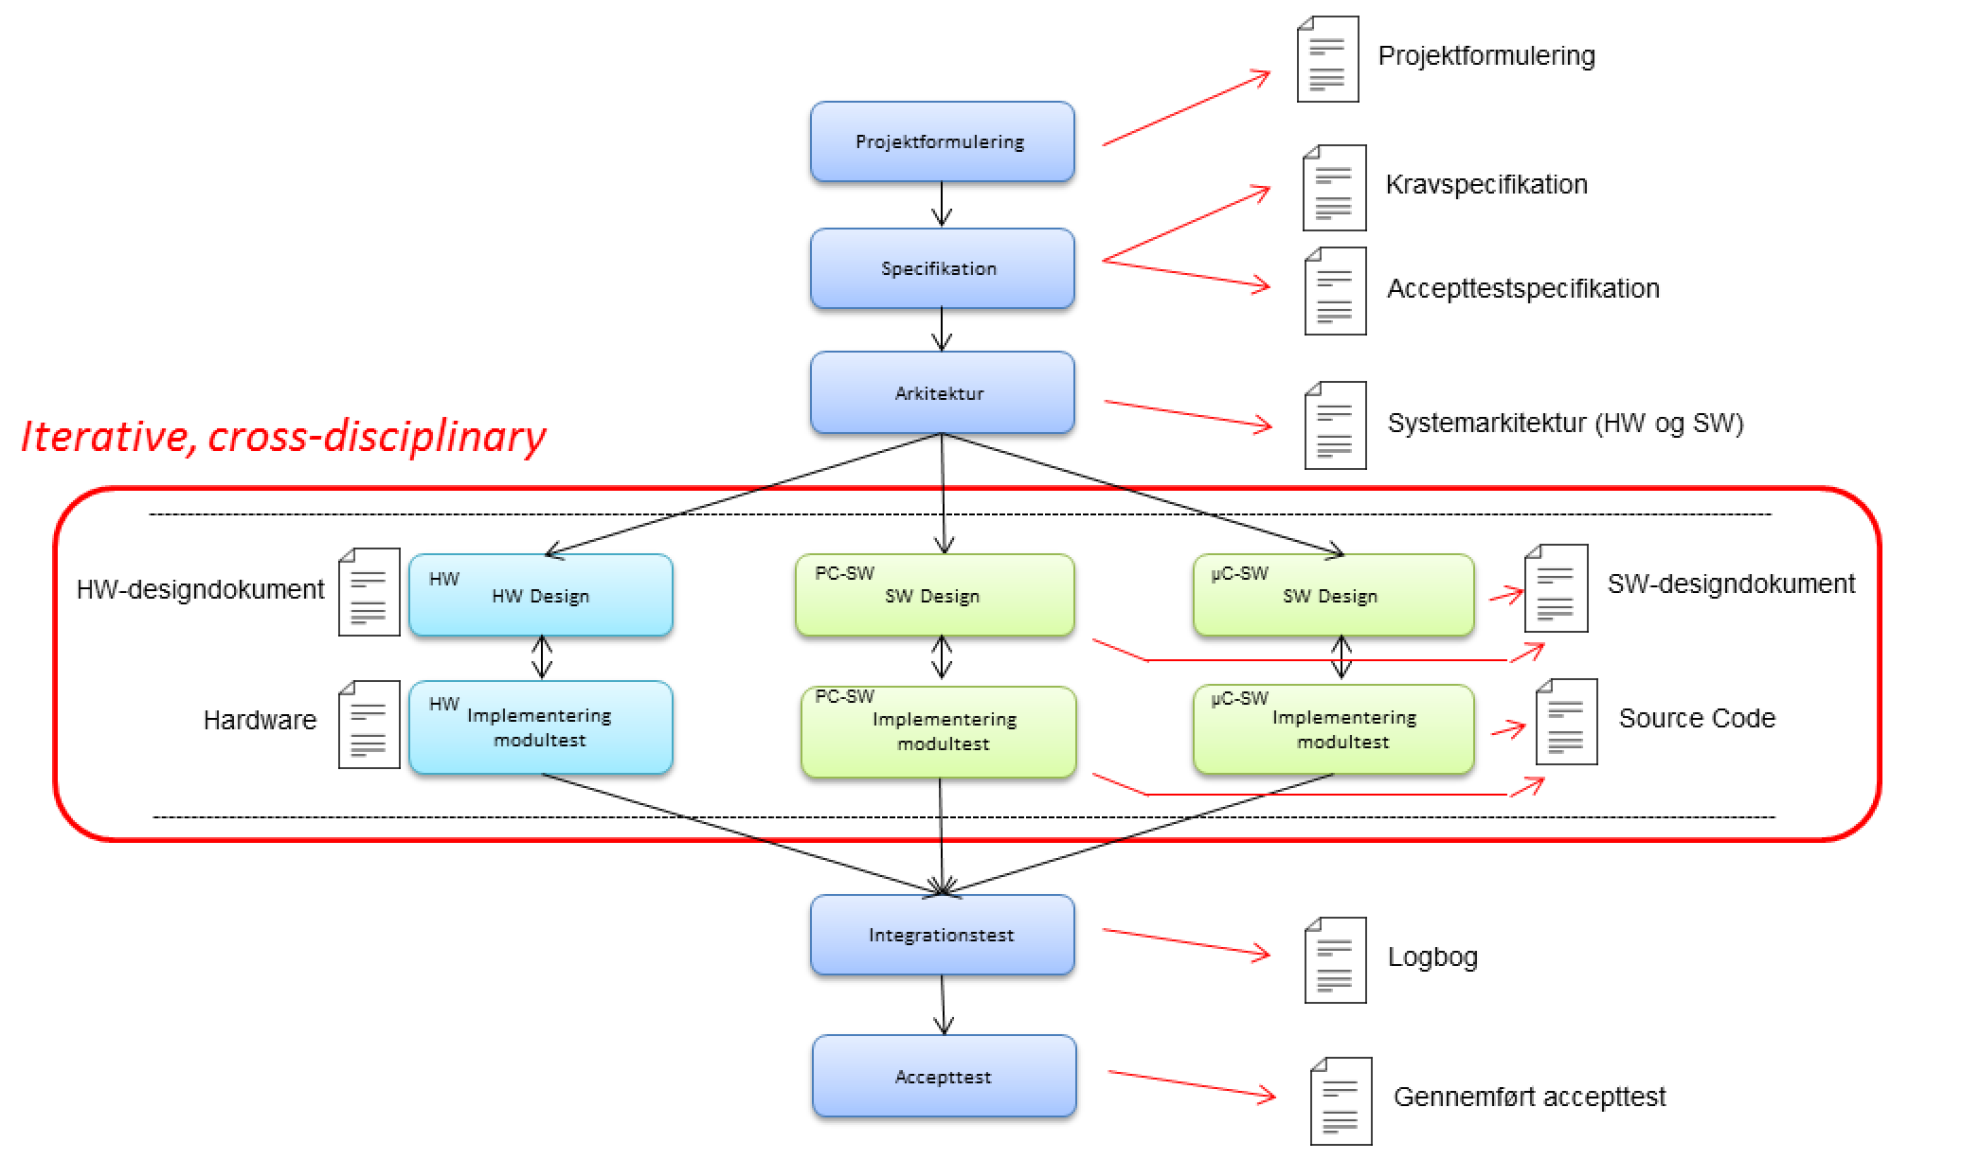
\includegraphics[max width=0.9\linewidth]{/tex/Metodeproces/billeder/ASEmodel.png}
	\caption{ASE model med fokus på iterativ proces}
	\label{fig:ASE}
\end{figure}  
\noindent I begyndelsen hvor produktets krav bliver specificeret, har processen ikke været så iterativt, som de efterfølgende faser. Det skyldes, at oplægget er kommet fra Terma. De har været med til at specificere kravene, som derfor har ligget forholdsvis fast. Der har været få ændringer løbende, men det er begrænset.

Til gengæld har især design-, implementerings- og testfasen fungeret iterativt. Her er produktet blevet forbedret af flere omgange. Inden hver iteration begyndes, gøres det klart, hvad der skal laves og hvad succeskriteriet er, inden næste iteration kan påbegyndes. 

\subsection{SysML}
Til at udarbejde systemarkitekturen for systemet, er der benyttet SysML. De anvendte SysML metoder for projektet har været block definitions diagrammer (BDD) og interne blok diagrammer (IBD). BDD'et er brugt til, at nedbryde systemerne i mindre blokke, som dermed skal give et bedre overblik over systemets dele. IBD'et viser den hardwaremæssige sammenhæng blokkene imellem.    

\noindent Ved at bruge SysML, er det nemmere for andre udviklere, at sætte sig ind i systemet. Samtidig gør det designfasen nemmere, når systemets virkemåde er fastlagt forinden.

\subsection{UML}
Ofte benyttes UML mest til analyse og udarbejdelse af softwarearkitekturen. I dette projekt er UML-metoden \textit{flowdiagram} istedet brugt til, at give et overblik over systemets ønskede virkemåde. Flowdiagrammer giver et overblik over de valg, systemet gennemgår, når det er aktivt.   

\subsection{MoSCoW} 
MoSCoW er en måde at prioritere krav på, alt efter hvor vigtige de er, for det samlede produkt.  
De stilles op i \textit{must}, som er krav, der skal overholdes. Næste prioritering er \textit{should}, som er krav, der bør overholdt. \textit{Could} er krav, der ville være gode til produktet, men som der ikke forventes, at være tid til at implementere. Sidste prioritering er \textit{won't}, hvilket er krav, som produktet ikke vil have. Med prioriteringen bør \textit{must} kravene være opfyldt, inden der kigges på \textit{should} kravene osv. 

\section{Proces}
Som beskrevet tidligere har udviklingsprocessen fungeret iterativt. Til at implementere udviklingsmodellen, er der brugt Scrum~\cite{Scrum}. Det er valgt, da det er et projektsstyringsværktøj, som begge medlemmer har haft succes med tidligere. Med en gruppe på to, er det ikke alle dele fra Scrum, som giver mening at bruge. Til dette projekt har det især været benyttet i forbindelse med daglige Scrum møder, og taskboards med backlog items. 

Til de daglige møder tages arbejdet fra dagen før op. Her forklares det, om man har været i stand til at udføre sine opgaver, og hvis ikke, hvilke problematikker det skyldes. Yderligere planlægges det, hvad der skal ske til næste gang. De daglige møder sørger for, at der bliver reflekteret over arbejdet løbende, hvilket sikrer, at valgene der tages er gennemtænkt. 

Hver fase fra ASE modellen er blevet anset som iterationer, og tildelt et taskboard hver. Hver iteration er delt op i mindre opgaver, der er lagt ind som backlog items på deres respektive taskboards. Design-, implementerings- og testiterationen er yderligere delt op i tre iterationer for at bevare overblikket. På figur~\ref{fig:Taskboard} ses et øjebliksbillede af taskboardet for 3. iteration af design, implementerings og test.
\begin{figure}[H]
	\center
	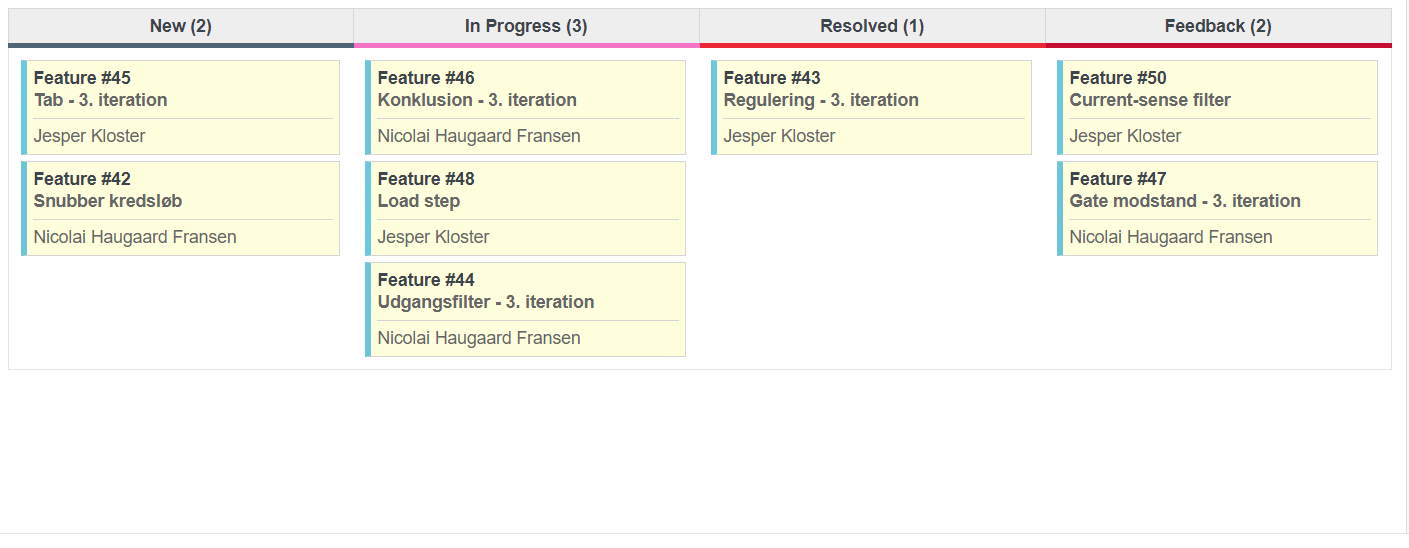
\includegraphics[max width=0.9\linewidth]{/tex/Metodeproces/Billeder/Scrumtask.png}
	\caption{Scrum taskboard}
	\label{fig:Taskboard}
\end{figure}        
\noindent Taskboardet sørger for, at give et overblik over hvilke opgaver, der er påbegyndt og hvilke der mangles. På den måde sikres det, at der ikke sidder to med samme opgave, eller opgaver der bliver forsømt.

Til konfigurationsstyring er der benyttet et repository over Github~\cite{Github}. Det er brugt til deling af dokumenter og versionshistorik af disse. Yderligere er rapport, dokumentation og procesbeskrivelse skrevet i programmet LaTeX~\cite{Latex}. Kombinationen mellem LaTeX og Github, gør det nemt at merge ændringer i dokumenterne. Det giver mulighed for, at ændre i dokumenterne samtidigt, uden det skaber problemer. Samtlige dokumenter og bilag, som er vedlagt, har været administreret over Github.
Den interne kommunikation i gruppen, er foregået over facebook. Det omhandler mødetidspunkter, spørgsmål og generelle informationer. Den eksterne kommunikation med vejleder og kontaktpersoner fra Terma, er foregået over mail.  

Der har i projektperioden været afholdt tre forskellige slags møder. De interne daglige møder, vejledermøde og eksterne møder med kontaktpersonerne fra Terma. 

Langt hen ad vejen har der været afholdt vejledermøder en gang i ugen. Her har der på forhånd været tilsendt dagsorden til vejlederen. Til møderne har der været en referent og en mødeleder, der sikrer, at dagsordenen overholdes. Disse roller er gået på skift fra møde til møde. Møderne har været brugt til, at diskutere arbejdet fra den forgangne uge og eventuelle opståede problemer. Derudover en forventning om opgaver, der skal udføres inden næste møde. De omdiskuterede problemer har både været faglige- og rapportmæssige. 

Der har været afholdt møder med kontaktpersonerne fra Terma næsten hver uge. Igen har der været sendt information til kontaktpersonerne forinden, for at give et overblik over, hvad der skal diskuteres. Møderne har været en god mulighed for, at diskutere de fagligt opståede udfordringer undervejs. Det er også her eventuelle ændringer af krav til produktet, har været diskuteret. Under design-, implementerings- og testiterationerne har der dagligt været faglige diskussioner. Det har været yderst produktivt, at kunne løse et eventuelt problem med det samme.

For yderligere information om den procesmæssige del af projektet, henvises til dokumentet "Procesbeskrivelse" i bilagsmappen.  